\section{Markt- und Wettbewerbsanalyse}
Die Marktanalyse kommerzieller Wortuhren dient der systematischen Untersuchung bestehender Produkte im Hinblick auf technische, funktionale und gestalterische Eigenschaften. 
Ziel ist die Identifikation aktueller Lösungsansätze, technologischer Standards sowie bestehender Einschränkungen. 
Die Analyse bildet eine fundierte Grundlage für die Ableitung eigener Systemanforderungen und unterstützt die Abgrenzung des geplanten Entwicklungsumfangs.

Der Markt für Wortuhren lässt sich grundsätzlich in mehrere Segmente unterteilen, die sich hinsichtlich Designanspruch, Funktionsumfang und Preisniveau unterscheiden. 

Im Premiumsegment dominieren Produkte wie die QLOCKTWO EARTH 45 des Herstellers Biegert\&Funk, die primär als Designobjekte positioniert sind~\cite{qlocktwo_earth45}. 
Diese Uhren bewegen sich typischerweise in einem Preisbereich von etwa 1.500 € bis über 3.000 €, abhängig von Größe und Materialausführung. 
Sie zeichnen sich durch hochwertige Materialien, minimalistische Gestaltung und eine klare Fokussierung auf die wortbasierte Zeitanzeige aus. 
Erweiterte Funktionen wie Wetterinformationen, Sensorintegration oder kontextbasierte Zusatzinformationen sind in diesem Segment kaum vorhanden. 
Trotz des hohen Preisniveaus resultiert daraus ein begrenzter funktionaler Mehrwert.

\begin{figure}[H]
	\centering
	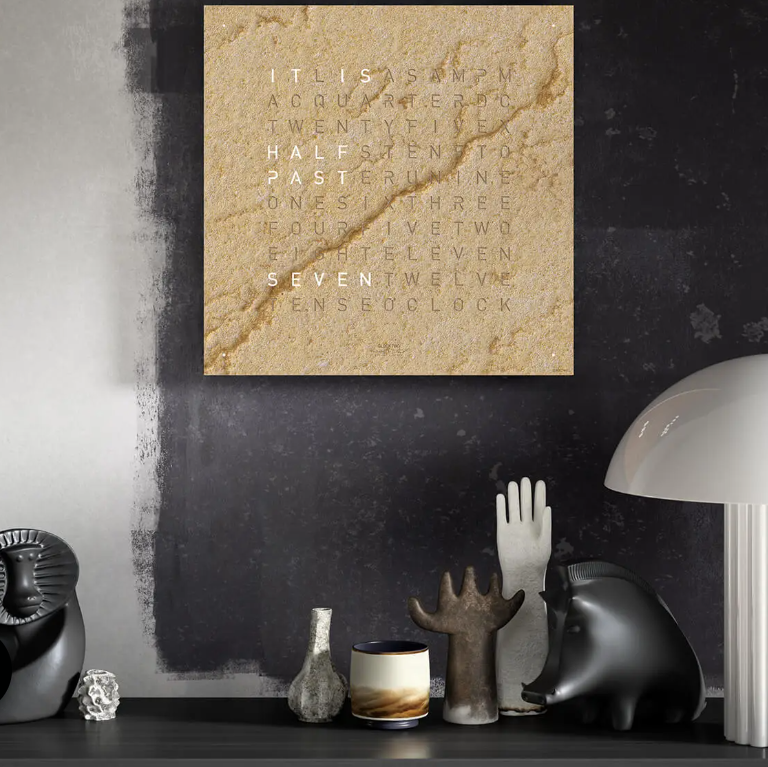
\includegraphics[width=0.5\linewidth]{inhalt/bilder/QlockTwoDessert.png}
	\caption{}
	\label{fig:qlocktwo_earth45}
\end{figure}

Im mittleren Preissegment finden sich technisch erweiterte Lösungen von Herstellern wie Build-Yours oder kleineren Anbietern im Bereich individualisierbarer LED-Wortuhren. 
Ein Beispiel hierfür ist die Wortuhr Jupiter, die je nach Ausführung in einem Preisbereich von etwa 200 € bis 600 € liegt~\cite{wordclock_jupiter}. 
Diese Systeme erweitern die klassische Wortuhr um grundlegende Funktionen wie WLAN-Anbindung, App-Steuerung oder Farbkonfiguration. 
Dadurch wird insbesondere die Individualisierung der Anzeige verbessert. 
Der Funktionsumfang bleibt jedoch überwiegend auf die Darstellung der Uhrzeit sowie visuelle Anpassungen beschränkt, während eine weitergehende Informationsintegration, beispielsweise durch externe Datenquellen, nur eingeschränkt umgesetzt wird.

\begin{figure}[H]
	\centering
	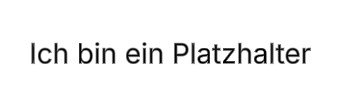
\includegraphics[width=0.5\linewidth]{inhalt/bilder/Platzhalter.jpg}
	\caption{}
	\label{fig:wordclock_jupiter}
\end{figure}

Demgegenüber stehen DIY- und Maker-Lösungen, die auf Mikrocontroller-Plattformen wie dem ESP32 basieren. 
Diese Systeme entstehen häufig in Community-getriebenen Projekten oder individuellen Entwicklungen. 
Die Materialkosten bewegen sich typischerweise im Bereich von etwa 50 € bis 200 €, abhängig von Komponenten wie LED-Matrix, Gehäuse und Sensorik. 
Diese Lösungen ermöglichen eine nahezu beliebige Erweiterung der Funktionalität, etwa durch die Einbindung von Wetterdaten, Temperaturmessung oder weiteren API-basierten Informationen~\cite{esp32_wordclock}. 
Allerdings weisen diese Systeme häufig Defizite hinsichtlich Gehäusedesign, Benutzerfreundlichkeit und Produktreife auf, wodurch sie für eine breitere Zielgruppe nur eingeschränkt geeignet sind.

\begin{figure}[H]
	\centering
	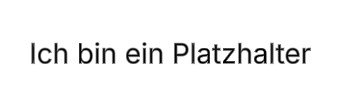
\includegraphics[width=0.5\linewidth]{inhalt/bilder/Platzhalter.jpg}
	\caption{}
	\label{fig:esp32_wordclock}
\end{figure}

Ein weiteres Segment bilden günstige Massenmarktprodukte, die über Onlineplattformen wie Alibaba oder vergleichbare Anbieter vertrieben werden~\cite{alibaba_wordclock}. 
Diese Produkte liegen preislich meist im Bereich von etwa 10 € bis 150 € und zeichnen sich durch eine einfache technische Umsetzung sowie eine stark reduzierte Funktionalität aus. 
Sie sind primär als dekorative Produkte einzuordnen und weisen sowohl in Bezug auf Materialqualität als auch Funktionsumfang deutliche Einschränkungen auf.

\begin{figure}[H]
	\centering
	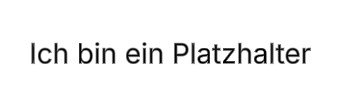
\includegraphics[width=0.5\linewidth]{inhalt/bilder/Platzhalter.jpg}
	\caption{}
	\label{fig:alibaba_wordclock}
\end{figure}

Zur systematischen Bewertung der betrachteten Systeme werden selbst definierte Kriterien verwendet. 
Neben funktionalen Eigenschaften werden der Kaufpreis sowie gestalterische Merkmale analysiert. 
Hierzu zählen insbesondere Materialwahl, Lichtcharakteristik, Formfaktor und Integrationsfähigkeit in Wohnumgebungen. 
Ein weiteres Kriterium stellt die zeitliche Präzision dar. 

Die Gegenüberstellung ermöglicht die Identifikation von Gemeinsamkeiten und Unterschieden zwischen den betrachteten Systemen. 
Auf dieser Grundlage lassen sich funktionale Defizite sowie Potenziale für Erweiterungen ableiten. 
Die gewonnenen Erkenntnisse fließen in die Konzeptionierung der im Rahmen dieser Arbeit entwickelten Wortuhr ein. 
Die Ergebnisse sind tabellarisch in Tabelle~\ref{tab:vergleich_wordclock_ohne_diy} dargestellt.

\begin{table}[h]
\centering
\begin{tabular}{|p{4cm}|p{3.5cm}|p{3.5cm}|p{3.5cm}|}
\hline
\textbf{Kriterium} & \textbf{Premium (z.\,B. QLOCKTWO / Biegert \& Funk)} & \textbf{Mittleres Segment (z.\,B. Build-Yours / Jupiter)} & \textbf{Massenmarkt (z.\,B. Alibaba)} \\
\hline
Preisbereich & ca. 1.500 € – 3.000 € & ca. 200 € – 600 € & ca. 10 € – 150 € \\
\hline
Zielsetzung & Designobjekt / Lifestyle & Kombination aus Technik \& Design & Dekorationsprodukt \\
\hline
Wortbasierte Zeitanzeige & o & o & o \\
\hline
Materialqualität & Sehr hoch (Metall, Holz) & Mittel bis hoch & Niedrig \\
\hline
Designfokus & Sehr hoch & Mittel & Gering \\
\hline
WLAN / Internet & x & o & x \\
\hline
App-Steuerung & x & o & x \\
\hline
Farb- / Anzeigeanpassung & x / sehr begrenzt & o & o (begrenzt) \\
\hline
Sekundenanzeige & o (teilweise) & x & x \\
\hline
Wetterdaten & x & x & x \\
\hline
Temperaturanzeige & x & x & x \\
\hline
Mondzeiten / Zusatzinfos & x & x & x \\
\hline
Erweiterbarkeit (APIs) & x & x & x \\
\hline
Benutzerfreundlichkeit & Sehr hoch & Hoch & Mittel \\
\hline
Produktreife & Sehr hoch & Hoch & Mittel \\
\hline
\end{tabular}
\caption{Vergleich verschiedener Wortuhren in verschiedenen Preissegmenten.}
\label{tab:vergleich_wordclock_ohne_diy}
\end{table}

Aus der Gegenüberstellung ergibt sich eine Diskrepanz zwischen Designqualität und funktionaler Leistungsfähigkeit. 
Im Premiumsegment zeigt sich trotz hoher Preise ein eingeschränkter Funktionsumfang.
Bei der QLOCKTWO CLASSIC ist z.B. eine Sekundenanzeige grundsätzlich möglich, erfordert jedoch dass diese durch drücken eines Knopfes ein- und ausgeschalten wird.
Die Sekundenanzeige erscheint dann als Ziffer durch gezieltes setzen der LEDs auf der Buchstabenmatrix, wodurch die Stundenanzeige unterbrochen ist~\cite{QlockTwoClassicSekundenanzeige}. 
Systeme im mittleren Preissegment bieten erste Ansätze technischer Erweiterungen, erreichen jedoch keine umfassende funktionale Integration moderner Informationssysteme. 
DIY-Systeme weisen eine hohe Funktionalität und Flexibilität bei vergleichsweise geringen Kosten auf, erfüllen jedoch häufig nicht die gestalterischen und konstruktiven Anforderungen eines marktfähigen Produkts.

% %%%%%%%%%%%%Unbearbeitet version, outdated, später löschen sobald neue abgenommen
% \section{Markt- und Wettbewerbsanalyse} \todo{text}
% Die Marktanalyse kommerzieller Wortuhren dient der Untersuchung bestehender Produkte im Hinblick auf technische, funktionale und gestalterische Eigenschaften. 
% Ziel ist die Identifikation aktueller Lösungsansätze, technologischer Standards sowie bestehender Einschränkungen. 
% Die Analyse bildet eine Grundlage für die Ableitung eigener Systemanforderungen und unterstützt die Abgrenzung des geplanten Entwicklungsumfangs.

% Der Markt für Wortuhren lässt sich grundsätzlich in mehrere Segmente unterteilen,die sich vor allem hinsichtlich Designanspruch, Funktionsumfang und Preisniveau unterscheiden. 
% Im Premiumsegment dominieren Produkte wie die QLOCKTWO EARTH 45 des Herstellers Biegert\&Funk, die primär als Designobjekte positioniert sind~\cite{qlocktwo_earth45}.
% Diese Uhren bewegen sich typischerweise in einem Preisbereich von etwa 1.500 € bis über 3.000 €, abhängig von Größe und Materialausführung. 
% Sie zeichnen sich durch hochwertige Materialien, minimalistische Gestaltung und eine klare Fokussierung auf die wortbasierte Zeitanzeige aus. 
% Erweiterte Funktionen wie Wetterinformationen, Sensorintegration oder kontextbasierte Zusatzinformationen sind in diesem Segment kaum vorhanden.
% Trotz des hohen Preisniveaus bieten diese Systeme somit nur einen begrenzten funktionalen Mehrwert.

% \begin{figure}[H]
% 	\centering
% 	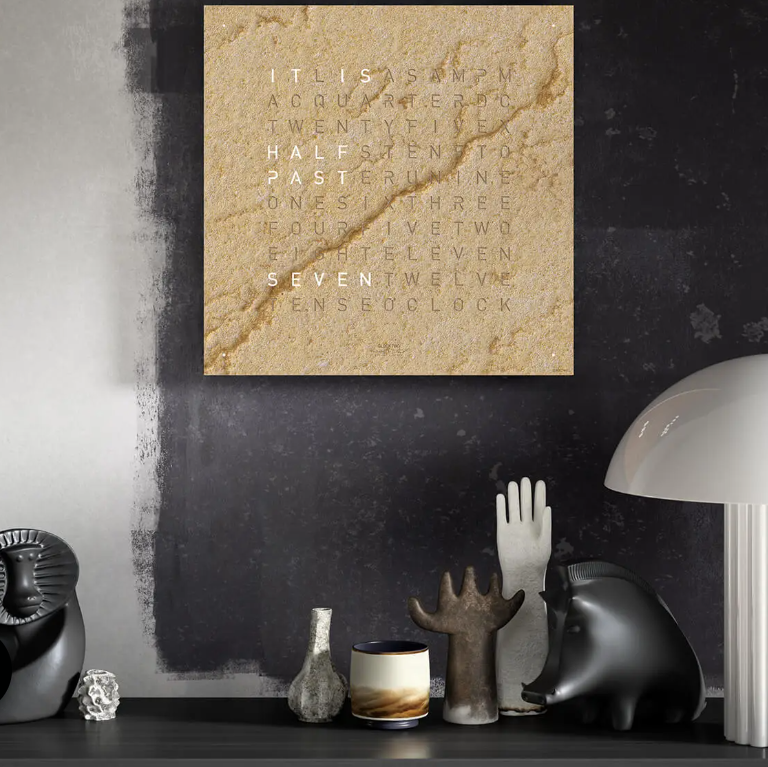
\includegraphics[width=0.5\linewidth]{inhalt/bilder/QlockTwoDessert.png}
% 	\caption{}
% 	\label{fig:qlocktwo_earth45}
% \end{figure}

% Im mittleren Preissegment finden sich zunehmend technisch orientierte Lösungen von Herstellern wie Build-Yours oder kleineren Anbietern im Bereich individualisierbarer LED-Wortuhren. 
% Ein Beispiel hierfür ist die Wortuhr Jupiter, die je nach Ausführung in einem Preisbereich von etwa 200 € bis 600 € liegt~\cite{wordclock_jupiter}. 
% Diese Systeme erweitern die klassische Wortuhr um grundlegende Funktionen wie WLAN-Anbindung, App-Steuerung oder Farbkonfiguration. 
% Dadurch wird insbesondere die Individualisierung der Anzeige verbessert. 
% Dennoch bleibt der Funktionsumfang meist auf die Darstellung der Uhrzeit sowie visuelle Anpassungen beschränkt, während weitergehende Informationsintegration, beispielsweise durch externe Datenquellen, nur eingeschränkt umgesetzt wird.

% \begin{figure}[H]
% 	\centering
% 	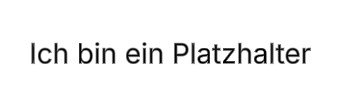
\includegraphics[width=0.5\linewidth]{inhalt/bilder/Platzhalter.jpg}
% 	\caption{}
% 	\label{fig:wordclock_jupiter}
% \end{figure}

% Demgegenüber stehen DIY- und Maker-Lösungen, die auf Mikrocontroller-Plattformen wie dem ESP32 basieren. 
% Diese Systeme sind nicht an klassische Hersteller gebunden, sondern entstehen häufig in Community-getriebenen Projekten und individuellen Entwicklungen. 
% Die Materialkosten bewegen sich typischerweise im Bereich von etwa 50 € bis 200 €, abhängig von Komponenten wie LED-Matrix, Gehäuse und Sensorik. 
% Diese Lösungen ermöglichen eine nahezu beliebige Erweiterung der Funktionalität, etwa durch die Einbindung von Wetterdaten, Temperaturmessung oder weiteren API-basierten Informationen~\cite{esp32_wordclock}. 
% Allerdings weisen diese Systeme häufig Defizite hinsichtlich Gehäusedesign, Benutzerfreundlichkeit und Produktreife auf, wodurch sie für eine breitere Zielgruppe nur eingeschränkt geeignet sind.

% \begin{figure}[H]
% 	\centering
% 	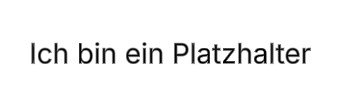
\includegraphics[width=0.5\linewidth]{inhalt/bilder/Platzhalter.jpg}
% 	\caption{}
% 	\label{fig:esp32_wordclock}
% \end{figure}

% Ein weiteres Segment bilden günstige Massenmarktprodukte, die über Onlineplattformen wie Alibaba oder vergleichbare Anbieter vertrieben werden~\cite{alibaba_wordclock}. 
% Diese Produkte liegen preislich meist im Bereich von etwa 10 € bis 150 € und zeichnen sich durch eine einfache technische Umsetzung sowie eine stark reduzierte Funktionalität aus. 
% Sie sind primär als dekorative Produkte einzuordnen und weisen sowohl in Bezug auf Materialqualität als auch Funktionsumfang deutliche Einschränkungen auf.

% \begin{figure}[H]
% 	\centering
% 	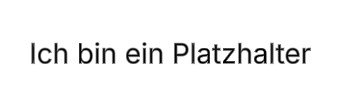
\includegraphics[width=0.5\linewidth]{inhalt/bilder/Platzhalter.jpg}
% 	\caption{}
% 	\label{fig:alibaba_wordclock}
% \end{figure}

% Die Untersuchung erfolgt anhand definierter Bewertungskriterien. 
% Neben funktionalen Eigenschaften werden der Kaufpreis sowie gestalterische Merkmale analysiert. 
% Hierzu zählen insbesondere Materialwahl, Lichtcharakteristik, Formfaktor und Integrationsfähigkeit in Wohnumgebungen. 
% Ein weiteres Kriterium stellt die zeitliche Präzision dar. 
% Dabei werden eingesetzte Zeitquellen, wie quarzbasierte Echtzeituhrmodule oder netzwerkbasierte Zeitsynchronisation, berücksichtigt. 

% Die systematische Gegenüberstellung ermöglicht die Identifikation von Gemeinsamkeiten und Unterschieden zwischen den betrachteten Systemen. 
% Auf dieser Grundlage lassen sich funktionale Defizite sowie Potenziale für innovative Erweiterungen ableiten. 
% Die gewonnenen Erkenntnisse fließen in die Konzeptionierung der im Rahmen dieser Arbeit entwickelten Wortuhr ein. 
% Die Ergebnisse sind tabellarisch in Tabelle~\ref{tab:vergleich_wordclock_ohne_diy} dargestellt.

% Aus der Gegenüberstellung ergibt sich eine deutliche Diskrepanz zwischen Designqualität und funktionaler Leistungsfähigkeit. 
% Insbesondere im Premiumsegment zeigt sich trotz hoher Preise ein eingeschränkter Funktionsumfang. 
% Systeme im mittleren Preissegment bieten erste Ansätze technischer Erweiterungen, erreichen jedoch keine umfassende funktionale Integration moderner Informationssysteme. 
% DIY-Systeme weisen hingegen eine hohe Funktionalität und Flexibilität bei vergleichsweise geringen Kosten auf, erfüllen jedoch häufig nicht die gestalterischen und konstruktiven Anforderungen eines marktfähigen Produkts.
% % Aus dieser Gegenüberstellung ergibt sich eine deutliche Diskrepanz zwischen Designqualität und funktionaler Leistungsfähigkeit. 
% % Die Tabelle 1 verdeutlicht, dass insbesondere im Premiumsegment trotz hoher Preise ein sehr eingeschränkter Funktionsumfang vorliegt. 
% % Systeme im mittleren Preissegment bieten erste Ansätze technischer Erweiterung, erreichen jedoch nicht die Tiefe funktionaler Integration moderner Informationssysteme. 
% % DIY-Systeme hingegen bieten ein hohes Maß an Funktionalität und Flexibilität bei vergleichsweise niedrigen Kosten, erreichen jedoch meist nicht die gestalterische und konstruktive Qualität eines marktfähigen Produkts.

% \begin{table}[h]
% \centering
% \begin{tabular}{|p{4cm}|p{3.5cm}|p{3.5cm}|p{3.5cm}|}
% \hline
% \textbf{Kriterium} & \textbf{Premium (z.\,B. QLOCKTWO / Biegert \& Funk)} & \textbf{Mittleres Segment (z.\,B. Build-Yours / Jupiter)} & \textbf{Massenmarkt (z.\,B. Alibaba)} \\
% \hline
% Preisbereich & ca. 1.500 € – 3.000 € & ca. 200 € – 600 € & ca. 10 € – 150 € \\
% \hline
% Zielsetzung & Designobjekt / Lifestyle & Kombination aus Technik \& Design & Dekorationsprodukt \\
% \hline
% Wortbasierte Zeitanzeige & o & o & o \\
% \hline
% Materialqualität & Sehr hoch (Metall, Holz) & Mittel bis hoch & Niedrig \\
% \hline
% Designfokus & Sehr hoch & Mittel & Gering \\
% \hline
% WLAN / Internet & x & o & x \\
% \hline
% App-Steuerung & x & o & x \\
% \hline
% Farb- / Anzeigeanpassung & x / sehr begrenzt & o & o (begrenzt) \\
% \hline
% Sekundenanzeige & o (teilweise) & x & x \\
% \hline
% Wetterdaten & x & x & x \\
% \hline
% Temperaturanzeige & x & x & x \\
% \hline
% Mondzeiten / Zusatzinfos & x & x & x \\
% \hline
% Erweiterbarkeit (APIs) & x & x & x \\
% \hline
% Benutzerfreundlichkeit & Sehr hoch & Hoch & Mittel \\
% \hline
% Produktreife & Sehr hoch & Hoch & Mittel \\
% \hline
% \end{tabular}
% \caption{Vergleich verschiedener Wortuhren in verschiedenen Preissegmenten.}
% \label{tab:vergleich_wordclock_ohne_diy}
% \end{table}

% %%%%%%%%%%%%%%%%%%%%%%%%%%%%%Tabelle mit ESP/DIY
% % \begin{table}[h]
% % \centering
% % \begin{tabular}{|p{4cm}|p{3cm}|p{3cm}|p{3cm}|p{3cm}|}
% % \hline
% % \textbf{Kriterium} & \textbf{Premium (z.\,B. QLOCKTWO / Biegert \& Funk)} & \textbf{Mittleres Segment (z.\,B. Build-Yours / Jupiter)} & \textbf{DIY / Maker (ESP32)} & \textbf{Massenmarkt (z.\,B. Alibaba)} \\
% % \hline
% % Preisbereich & ca. 1.500 € – 3.000 € & ca. 200 € – 600 € & ca. 50 € – 200 € & ca. 10 € – 150 € \\
% % \hline
% % Zielsetzung & Designobjekt / Lifestyle & Kombination aus Technik \& Design & Technische Plattform & Dekorationsprodukt \\
% % \hline
% % Wortbasierte Zeitanzeige & o & o & o & o \\
% % \hline
% % Materialqualität & Sehr hoch (Metall, Holz) & Mittel bis hoch & Variabel & Niedrig \\
% % \hline
% % Designfokus & Sehr hoch & Mittel & Gering & Gering \\
% % \hline
% % WLAN / Internet & x & o & o & x \\
% % \hline
% % App-Steuerung & x & o & o (optional) & x \\
% % \hline
% % Farb- / Anzeigeanpassung & x / sehr begrenzt & o & o & o (begrenzt) \\
% % \hline
% % Sekundenanzeige & o (teilweise) & x & o & x \\
% % \hline
% % Wetterdaten & x & x & o & x \\
% % \hline
% % Temperaturanzeige & x & x & o & x \\
% % \hline
% % Mondzeiten / Zusatzinfos & x & x & o & x \\
% % \hline
% % Erweiterbarkeit (APIs) & x & x & o & x \\
% % \hline
% % Benutzerfreundlichkeit & Sehr hoch & Hoch & Mittel & Mittel \\
% % \hline
% % Produktreife & Sehr hoch & Hoch & Niedrig & Mittel \\
% % \hline
% % \end{tabular}
% % \caption{Vergleich verschiedener WordClock-Segmente}
% % \label{tab:vergleich_wordclock}
% % \end{table}

% Vor diesem Hintergrund gewinnt die Entwicklung einer eigenen Wortuhr besondere Relevanz. 
% Ziel ist es, die bestehenden Schwächen der aktuellen Marktsegmente zu überwinden, indem eine Lösung geschaffen wird, die sowohl gestalterische als auch funktionale Anforderungen vereint. 
% Die entwickelte Wortuhr integriert neben der klassischen wortbasierten Zeitanzeige zusätzliche Funktionen wie Sekundenanzeige, Wetterdaten, Temperaturinformationen und Mondzeiten. 
% Durch den Einsatz eines internetfähigen Mikrocontrollers wird zudem die Grundlage für eine erweiterbare und zukunftsfähige Systemarchitektur geschaffen.

% Die Bewertung in der unterstehenden Tabelle~\ref{tab:bewertung_wordclock} zeigt, dass bestehende Systeme entweder in einzelnen Kategorien sehr stark sind, jedoch keine ganzheitlich ausgewogene Lösung darstellen. 
% Premiumprodukte erreichen hohe Werte im Bereich Design und Benutzerfreundlichkeit, schneiden jedoch im Funktionsumfang und in der Erweiterbarkeit schwach ab. 
% DIY-Systeme hingegen überzeugen durch hohe Funktionalität und Erweiterbarkeit, weisen jedoch Defizite im Design und in der Benutzerfreundlichkeit auf. 
% Die entwickelte Wortuhr erreicht hingegen in allen Kategorien hohe Bewertungen und stellt somit eine ausgewogene und leistungsfähige Gesamtlösung dar.

% \begin{table}[h]
% \centering
% \begin{tabular}{|c|c|c|c|c|c|c|}
% \hline
% \textbf{Produkt} & \textbf{Design} & \textbf{Funktion} & \textbf{Usability} & \textbf{Erweiterbarkeit} & \textbf{Preis-Leistung} & \textbf{Gesamt} \\
% \hline
% QLOCKTWO & 5 & 2 & 5 & 1 & 2 & 3,05 \\
% \hline
% Jupiter & 3 & 3 & 4 & 2 & 3 & 3,05 \\
% \hline
% Massenmarkt & 2 & 1 & 3 & 1 & 4 & 2,10 \\
% \hline
% Eigene Wortuhr & 4 & 5 & 4 & 5 & 4 & 4,45 \\
% \hline
% \end{tabular}
% \caption{Bewertung verschiedener WordClock-Konzepte}
% \label{tab:bewertung_wordclock}
% \end{table} \todo{Tabelle überarbeiten und page matching}

% %%%%%%%%%%%%%%%%%%%Tabelle mit ESP/DIY
% % \begin{table}[h]
% % \centering
% % \begin{tabular}{|c|c|c|c|c|c|c|}
% % \hline
% % \textbf{Produkt} & \textbf{Design} & \textbf{Funktion} & \textbf{Usability} & \textbf{Erweiterbarkeit} & \textbf{Preis-Leistung} & \textbf{Gesamt} \\
% % \hline
% % QLOCKTWO & 5 & 2 & 5 & 1 & 2 & 3,05 \\
% % \hline
% % Jupiter & 3 & 3 & 4 & 2 & 3 & 3,05 \\
% % \hline
% % DIY (ESP32) & 2 & 5 & 2 & 5 & 5 & 3,70 \\
% % \hline
% % Massenmarkt & 2 & 1 & 3 & 1 & 4 & 2,10 \\
% % \hline
% % Eigene Wortuhr & 4 & 5 & 4 & 5 & 4 & 4,45 \\
% % \hline
% % \end{tabular}
% % \caption{Bewertung verschiedener WordClock-Konzepte}
% % \label{tab:bewertung_wordclock}
% % \end{table}

% Damit positioniert sich die entwickelte Lösung zwischen den bestehenden Marktsegmenten und adressiert gezielt eine bislang nur unzureichend besetzte Nische. 
% Sie stellt nicht nur eine technische Erweiterung bestehender Systeme dar, sondern verfolgt den Ansatz, die Wortuhr von einem reinen Designobjekt zu einem intelligenten Informationssystem weiterzuentwickeln. 
% Diese Kombination aus ästhetischer Gestaltung und funktionaler Erweiterbarkeit begründet die Relevanz der eigenen Entwicklung sowohl aus technischer als auch aus marktbezogener Perspektive.


% % Im Fokus stehen dabei vier kommerziell vertrieben Wortuhren unterschiedlicher Hersteller:innen und Preissegmente. 
% % Die Untersuchten Wortuhren sind in Abbildung~\ref{fig:VergleichWortuhren} dargestellt.
% % \begin{figure}[H]
% %     \centering
% %     \begin{subfigure}[t]{0.35\textwidth}
% %         \centering
% %         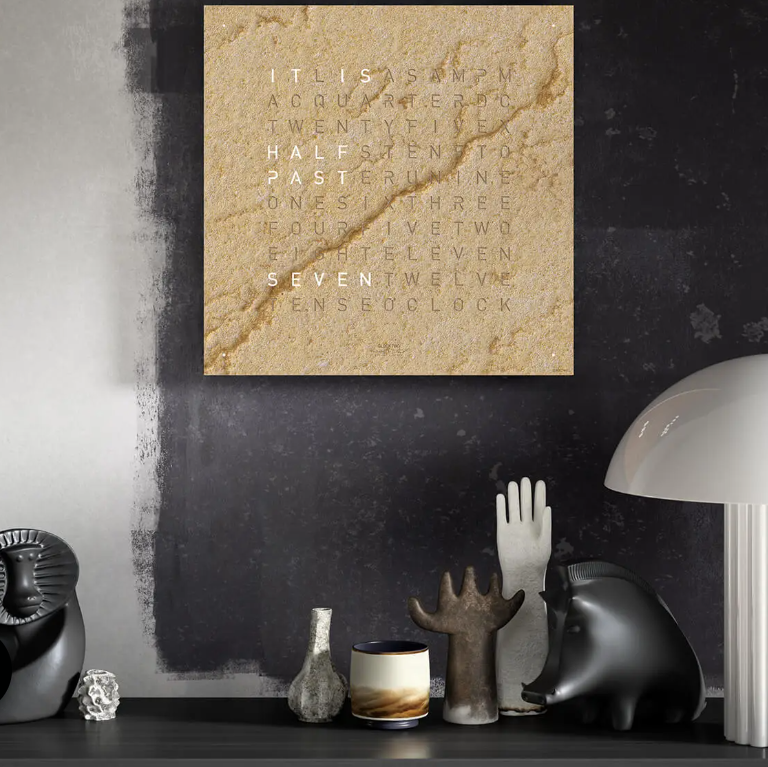
\includegraphics[width=\linewidth]{inhalt/bilder/QlockTwoDessert.png}
% %         \caption{Das Model Earth 45 von QlockTwo mit deutschem Text im Design Dessert~\cite{QlockTwoDesert}.}
% % 	    \label{fig:QlockTwoDessert}
% %     \end{subfigure}
% %     \hfill
% %     \begin{subfigure}[t]{0.35\textwidth}
% %         \centering
% %         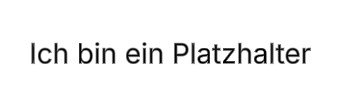
\includegraphics[width=\linewidth]{inhalt/bilder/Platzhalter.jpg}
% %         \caption{rechts oben.}
% %         \label{fig:sub1_b}
% %     \end{subfigure}
% %     \vspace{0.8em}
% %     \begin{subfigure}[t]{0.35\textwidth}
% %         \centering
% %         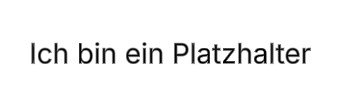
\includegraphics[width=\linewidth]{inhalt/bilder/Platzhalter.jpg}
% %         \caption{links unten.}
% %         \label{fig:sub1_c}
% %     \end{subfigure}
% %     \hfill
% %     \begin{subfigure}[t]{0.35\textwidth}
% %         \centering
% %         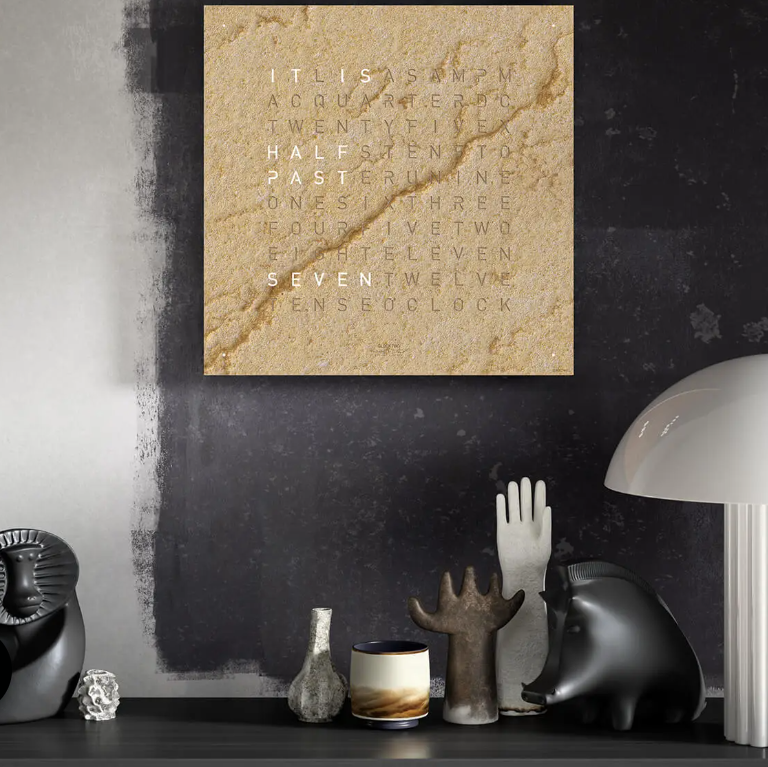
\includegraphics[width=\linewidth]{inhalt/bilder/QlockTwoDessert.png}
% %         \caption{rechts unten.}
% %         \label{fig:sub1_d}
% %     \end{subfigure}
% %     \caption{Vergleich von vier kommerziell vertriebenen Wortuhren verschiedener Hersteller:innen.}
% %     \label{fig:VergleichWortuhren}
% % \end{figure}

% % Abbildung~\ref{fig:QlockTwoDessert} zeigt das Model Earth 45 des Herstellers Qlocktwo im Design Desert in deutscher Sprache.
% % % Hier text welche 4 und warum, darunter bild mit 4 subfigures je eine Uhr.
% % Diese Produkte repräsentieren verschiedene Marktsegmente hinsichtlich Kosten, Funktionsumfang und technischer Ausführung. 

% % Die Untersuchung erfolgt anhand selbst definierter Bewertungskriterien. 
% % Neben funktionale Eigenschaften werden auch der Kaufpreis und gestalterische Merkmale analysiert. 
% % Darunter Materialwahl, Lichtcharakteristik, Formfaktor und Integrationsmöglichkeiten in Wohnumgebungen. 
% % Ein weiteres Kriterium stellt die zeitliche Präzision dar. 
% % Hierbei werden eingesetzte Zeitquellen, beispielsweise quarzbasierte Echtzeituhrmodule oder netzwerkbasierte Zeitsynchronisation, betrachtet. 

% % Die Gegenüberstellung ermöglicht die Identifikation von Gemeinsamkeiten und Unterschieden zwischen den betrachteten Systemen. 
% % Auf dieser Basis lassen sich funktionale Defizite sowie Potenziale für innovative Erweiterungen ableiten. 
% % Die gewonnenen Erkenntnisse fließen in die Konzeptionierung der im Rahmen dieser Arbeit entwickelten Wortuhr ein.
% % Die Ergebnisse sind Tabellarisch in Tabelle~\ref{tab:VergleichWortuhren} dargestellt.